\documentclass[letter, 10pt]{article}
\usepackage[utf8]{inputenc}
\usepackage[spanish, es-tabla]{babel}
\usepackage{amsfonts}
\usepackage{amsmath}
\usepackage[dvips]{graphicx}
\usepackage{graphicx}
\usepackage{subfigure} % subfiguras
\DeclareGraphicsExtensions{.bmp,.png,.pdf,.jpg}
\usepackage{xcolor,listings}%color support for listings
\usepackage{epstopdf}
\usepackage{algpseudocode}
\usepackage{algorithm}
\usepackage{url}
\usepackage{caption}
\usepackage{cite}
\usepackage[top=3cm,bottom=3cm,left=3.5cm,right=3.5cm,footskip=1.5cm,headheight=1.5cm,headsep=.5cm,textheight=3cm]{geometry}



\begin{document}



\title{Análisis Inteligente de Datos \\ \begin{Large}Tarea 2\end{Large}}
\author{Paulina Aguila - Juan Avalo}
\date{23 de junio de 2016}

\maketitle


\begin{figure}[ht]
\begin{center}

\includegraphics[width=0.2\textwidth]{Images/Isotipo-Negro.png}\\
\end{center}
\end{figure}
\vspace{2cm}
\section{Introducci\'on}
ACA INTRO

\section{Regresión Lineal Ordinaria (LSS)}

En esta sección, se estudiará un dataset llamado \textit{prostate-cancer}\cite{D}, que se utiliza a menudo con métodos de regresión. Los datos corresponden a un estudio realizado por Tom Stamey (Universidad de Stanford) en 1989 referente a la posible correlación entre el nivel de antígeno prostático específico (PSA) medido en un paciente, y otras mediciones clínicas que se obtuvieron luego de extirpar totalmente la próstata y los tejidos circundantes. Una de las variables que se estudian corresponden al volumen del cáncer prostático detectado en el paciente.

\subsection{Descripción de los datos}
En base al dataset, se construye con Python un dataframe de dimensión (97,9), es decir, de 9 variables y 97 datos. A continuación, se describen las variables \cite{DD}:

\begin{itemize}
\item \textbf{Lcavol: }Variable cuantitativa continua que representa el registro del volumen del cáncer. Toma valores flotantes desde -1,347 hasta 3,821.
\item \textbf{Lweight: }Variable cuantitativa continua que registra el valor del peso de la próstata. Toma valores flotantes desde 2,375 hasta 4,780. 
\item \textbf{Age: }Variable cuantitativa de tipo continua que representa la edad en años de la persona. Toma valores enteros desde 41 hasta 79 años.
\item \textbf{Lbph: }Variable cuantitativa continua que registra la cantidad de hiperplasia prostática benigna (HBP)\footnote{La hiperplasia benigna de próstata (HBP) es un agrandamiento no canceroso de la glándula prostática cuya prevalencia aumenta progresivamente con la edad.}. Toma valores flotantes desde -1,386 hasta 2,326. 
\item \textbf{Svi: }Variable categórica binaria que representa si existe invasión del cáncer en la vesícula seminal\footnote{Las vesículas o glándulas seminales son las encargadas de producir el 60\% del volumen del líquido seminal. Están ubicadas por encima de la base de la próstata, con la que están unidas por su extremo inferior.}. Toma los siguientes valores: 0: No hay invasión - 1: Si hay invasión. 
\item \textbf{Lcp: }Variable cuantitativa de tipo continua que representa el registro de penetración capsular\footnote{La próstata posee una fina envoltura que se conoce como cápsula prostática que define su límite. La penetración capsular es cuando las células cancerígenas se extienden y cruzan dicha envoltura.}. Toma valores flotantes entre -1,386 y 2,904. 
\item \textbf{Gleason: }Variable categórica ordinal que contiene el puntaje de Gleason\footnote{La escala de Gleason es un sistema que se emplea para medir el grado de agresividad de un cáncer de próstata, basándose en la observación de una muestra de biopsia. Si toma valores entre 2 y 6 corresponde a un cáncer con escasa agresividad, si toma valor 7 es un cáncer con agresividad intermedia, mientras que, si es de 8 a 10, corresponde a un cáncer de alta agresividad y peor pronóstico.}. Toma valores enteros entre 6 y 9.
\item \textbf{Pgg45: }Variable cuantitativa continua que representa el porcentaje del patrón de Gleason 4 y 5\footnote{El porcentaje del patrón de Gleason 4/5 se obtiene agregando los porcentajes de los patrones 4 y 5 de Gleason, es decir, la proporción combinada del tumor compuesto por el patrón 4 o el patrón 5 de Gleason, o ambos.}. Toma valores enteros entre 0 y 100.
\item \textbf{Lpsa: }Variable cuantitativa continua que corresponde al registro del análisis del antígeno prostático específico (PSA)\footnote{El antígeno prostático específico, o PSA, es una proteína producida por las células de la glándula prostática. El análisis del PSA mide la concentración del PSA en la sangre de un hombre. La concentración del PSA en la sangre es frecuentemente elevada en hombres con cáncer de próstata.}. Toma valores flotantes entre -0,430 hasta 5,583.
\item \textbf{Train: }Variable categórica nominal que representa si el dato es de tipo Test o de Training. Del total de 97 datos, 67 de ellos corresponden a datos de entrenamiento, mientras que 30 son datos de prueba. Toma los siguientes valores: T: Training set - F: Test set.
\end{itemize}

\subsection{Desarrollo}
Para comenzar con el desarrollo de la regresión lineal, en primer lugar, se deben normalizar los datos. Este es un paso muy importante, ya que permite ajustar la escala de las variables a la varianza de la unidad, lo que hace que los valores de datos que se encuentran ubicados en los extremos, no ejerzan un peso excesivo en la función objetivo.\\

Luego, al dataset se le debe quitar la columna \textbf{lpsa}, ya que esta formaría el vector y que corresponde a la función que se desea predecir. Al último dataframe, se le inserta una nueva columna llamada \textbf{intercept} compuesta solo de unos. Esto se realiza para que el modelo (ecuación) tenga un desplazamiento constante, el que actúa como intercepción \cite{P2}. Además, si se realiza el ajuste sin esa columna de unos, puede ocurrir que el coeficiente de determinación ($R^2$) pueda ser menor que cero. Es fácil de entender: puede que los regresores ensayados no den cuenta de la variabilidad de $\vec{y}$, y $SSE$ sea por tanto grande. Si acontece que $\vec{y}$ tiene poca variabilidad en torno a su media, $SST$ será en cambio pequeño, y $SST-SSE$ puede fácilmente ser negativo \cite{P1}.\\

Luego, de realizar estos pasos, se realiza una regresión lineal de mínimos cuadrados básica, para la cual se obtienen los valores del z-score y los pesos para cada variable. Para el cálculo del z-score, se realiza lo siguiente:

\begin{equation}
z_j=\frac{\hat{\beta }_j}{\hat{\sigma }\sqrt{v_j}}
\end{equation}

En donde, $\hat{\beta }_j$ son los coeficientes estimados por la regresión lineal del atributo $j$, $\hat{\sigma }$ corresponde a la desviación estándar estimada y $v_j$ es el $j$-ésimo elemento de $\left ( X^{T}X \right )^{-1}$. El iterador $j$ recorre todo el universo de atributos, por lo que en este caso $j=1,2,...,9$. La Tabla \ref{zscore} muestra un resumen con los valores obtenidos para cada variable.

\begin{table}[!hbt] 
\begin{center}
\begin{tabular}{| c | r | r |} 
\hline
\textbf{Variable} & \textbf{Peso} & \textbf{Z Score}\\ 
\hline 
lcavol & 0.676 & 5.319\\ 
lweight &0.261 & 2.727\\
age &-0.141 & -1.384\\
lbph &0.209 & 2.038\\
svi & 0.304& 2.448\\
lcp & -0.287& -1.851\\
gleason & -0.021& -0.145\\
pgg45 &0.266 &  1.723\\
intercept &2.465 & 27.359\\
\hline 
\end{tabular}
\caption{Recuadro con los coeficientes (pesos) y el valor del Z Score para cada variable.} 
\label{table:zscore}
\end{center} 
\end{table}

Dada la Tabla \ref{zscore}, se puede saber qué variables están más correlacionadas con la respuesta en base al valor que toma Z-Score, ya que las variables que tienen los mayores valores en valor absoluto del Z-Score, son las que más importancia y correlación tienen, por lo que son las que se deben seleccionar. En este caso, las variables más significativas por orden de importancia serían \textbf{lcavol}, \textbf{lweight}, \textbf{svi} y \textbf{lbph}. Esto tiene mucho sentido, ya que \textbf{lcavol} corresponde al volumen del cáncer, por lo que mientras más grande sea, mayor es la probabilidad de que tenga más PSA en la sangre. Al existir un Z-Score mayor que 2 en valor absoluto, esto quiere decir que la variable es significativa al nivel del 5\%, por lo que las variables menores a 2, como son \textbf{age}, \textbf{lcp}, \textbf{gleason} y \textbf{pgg45}.\\

Luego, se aplica Validación Cruzada o \textit{Cross Validation} con 5 y 10 bloques (k-folds) sobre los datos de entrenamiento, esto quiere decir, que los datos se dividen en 5 o 10 cajas. Para esto, es necesario realizar el ajuste de regresión lineal cada vez que se cambia el número de folds para que la estimación sea razonable. La Tabla \ref{msecross} muestra un resumen de los errores de predicción obtenidos.

\begin{table}[!hbt] 
\begin{center}
\begin{tabular}{| l | c |} 
\hline
\textbf{Set} & \textbf{Error}\\ 
\hline 
Test & 0.521\\ 
Training k=5 &0.957\\
Training k=10 &0.757\\
\hline 
\end{tabular}
\caption{Resumen con los errores de predicción para datos de test y training con validación cruzada.} 
\label{table:msecross}
\end{center} 
\end{table}

De la Tabla \ref{msecross}, se puede observar que para los datos de entrenamiento mientras más cantidad de bloques se utilicen en la validación cruzada, menor será el error de predicción obtenido, pero así mismo también aumentará la complejidad del algoritmo, dado que, si se aumenta la cantidad de k de tal forma que sea del mismo tamaño que la cantidad de datos, se obtendrá un error muy similar al real sin validación cruzada. Por otra parte, si se analiza el error del conjunto de prueba, se ve que el error es mucho menor. Este efecto se debe a la falta de regularización, ya que en validación cruzada se puede producir subajuste (underfitting) o sobreajuste (overfitting).\\

Se realiza un gráfico llamado ``quantile-quantile plot" para poder analizar si tiene sentido la hipótesis de que los residuos del modelo siguen una distribución normal. El gráfico se puede ver en la Figura \ref{qqplot}.

\begin{figure}[h]
\begin{center}
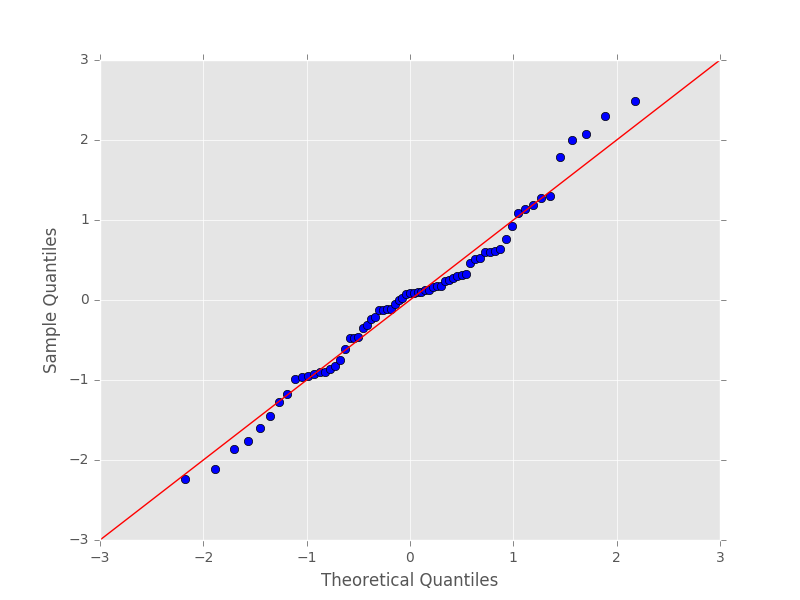
\includegraphics[width=0.7\textwidth]{Images/grafico1-j.png}
\caption{Histograma correspondiente a la cantidad de fallecidos y sobrevivientes de acuerdo a la variable edad.}
\label{qqplot}
\end{center}
\end{figure}

Del gráfico, se puede ver que sí se puede afirmar que tenga sentido que los residuos sigan una distribución normal, ya que los datos de la predicción (en azul), tienden a seguir la línea de los teóricos. Además, se observa que en el centro existe una tendencia que puede verse como una campana gaussiana.

\section{Selección de Atributos}

\section{Regularización}

\section{Predicción de Utilidades de Películas}

\section{Conclusiones}

ACA CONCLUSIONES

\bibliographystyle{plain}
\bibliography{Referencias}

\end{document} 